\documentclass[11pt,english]{article}

\usepackage[english]{babel}
\usepackage{enumitem}
\usepackage{fancyhdr}
\usepackage[top=2.3cm, bottom=2.3cm, left=1.6cm, right=1.6cm]{geometry}
\usepackage{graphicx}
\usepackage{lastpage}
\usepackage{tabularx}

\pagestyle{fancy}
\setlength{\parindent}{0pt}        % indentation on new paragraph
\setlength{\parskip}{0pt}          % vertical spacing on new paragraph
\setlength{\lineskip}{1pt}         % vertical spacing between lines
\setlength{\columnsep}{1cm}        % spacing between columns
\setlength{\belowcaptionskip}{0pt} % spacing below captions
\setlength{\abovecaptionskip}{5pt} % spacong above captions

\graphicspath{{assets/}}

\lfoot{}
\cfoot{\today}
\rfoot{\thepage/\pageref{LastPage}}

\newcommand*{\Frontpage}{\begingroup
	\hbox{%
		\hspace*{0.2\textwidth}
		\rule{1pt}{\textheight}
		\hspace*{0.05\textwidth}
		\parbox[b]{0.75\textwidth}{%
			{\noindent\Huge\bfseries DATAB3}\\[2\baselineskip] % Title
			{\large \textit{Huiswerkopdrachten}}\\[4\baselineskip] % Tagline or further description
			{\Large \textsc{\\
				Patrick Spek, 2099745 \\
				Chris Meesters, 2098474 \\
			}}
			\vspace{0.5\textheight} % Whitespace between the title block and the publisher
		}
	}
\endgroup}

\renewcommand{\footrulewidth}{0.4pt}

\begin{document}
	\thispagestyle{empty}
	\Frontpage

	\newpage
	\tableofcontents

	\newpage
	\section{Schermafdrukken}
	\subsection{Desktop}
	\makebox[\textwidth]{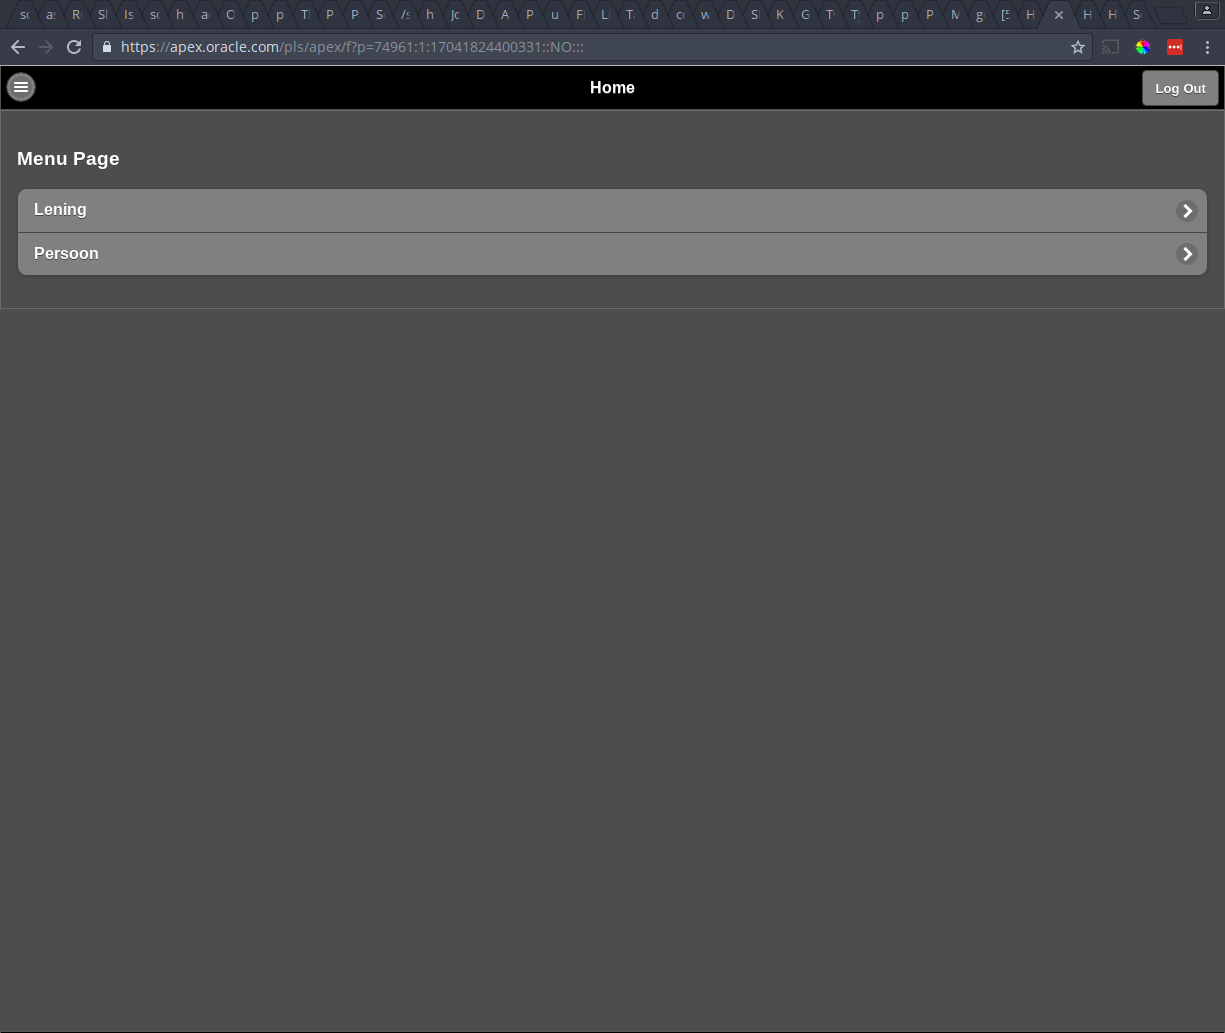
\includegraphics[width=\linewidth]{scrot-laptop}}

	\subsection{Mobile}
	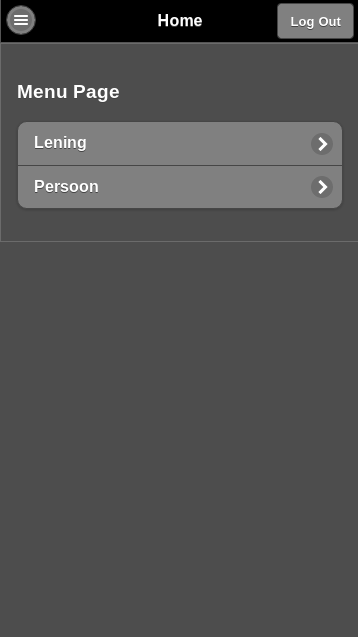
\includegraphics[scale=0.5]{scrot-mobile}

	\newpage
	\section{Contextdiagram}
	\makebox[\textwidth]{\includegraphics[width=\linewidth]{context}}

	\newpage
	\section{Use cases}
	\subsection{Aanvragen van een lening}
	\begin{tabularx}{\textwidth}{ l | X }
		\textbf{Use case nummer} & 1 \\
		\textbf{Naam} & Aanvragen van een lening \\
		\textbf{Scenario} &
		\begin{enumerate}
			\item Gebruiker logt in op systeem
			\item Gebruiker kiest nieuwe lening
			\item Systeem toont mogelijke uitleners
			\item Gebruiker kiest een uitlener
			\item Systeem vraagt bedrag
			\item Gebruiker vult bedrag in
			\item Systeem maakt lening aan
			\item Systeem schrijft geld over van uitlener naar gebruiker
		\end{enumerate} \\
		\textbf{Output} & Gebruiker heeft een nieuwe lening geopened.
	\end{tabularx}

	\newpage
	\subsection{Afbetalen van een lening}
	\begin{tabularx}{\textwidth}{ l | X }
		\textbf{Use case nummer} & 2 \\
		\textbf{Naam} & Afbetalen van een lening \\
		\textbf{Scenario} &
		\begin{enumerate}
			\item Gebruiker logt in op systeem
			\item Gebruiker kiest lening afbetalen
			\item Systeem berekent rente
			\item Systeem geeft totale kosten weer
			\item Gebruiker voert in dat de lening betaald is
			\item Systeem geeft aan dat de lening is afbetaal
		\end{enumerate} \\
		\textbf{Output} & Gebruiker heeft zijn lening afbetaald
	\end{tabularx}

	\newpage
	\subsection{Overzicht van leningen opvragen}
	\begin{tabularx}{\textwidth}{ l | X }
		\textbf{Use case nummer} & 3 \\
		\textbf{Naam} & Overzicht van leningen opvragen \\
		\textbf{Scenario} &
		\begin{enumerate}
			\item Beheerder logt in op systeem
			\item Beheerder kiest leningoverzicht
			\item Systeem geeft overzicht van alle lopende leningen weer
		\end{enumerate} \\
		\textbf{Output} & Gebruiker heeft zijn lening afbetaald
	\end{tabularx}

	\newpage
	\subsection{Systeem opschonen}
	\begin{tabularx}{\textwidth}{ l | X }
		\textbf{Use case nummer} & 4 \\
		\textbf{Naam} & Systeem opschonen \\
		\textbf{Scenario} &
		\begin{enumerate}
			\item Nieuwe maand begint
			\item Systeem verwijdert alle afbetaalde leningen uit de database
			\item Systeem verwijdert alle overbodige personen uit de database
			\item Systeem stuurt bericht aan beheerder
		\end{enumerate} \\
		\textbf{Output} & Overbodige personen en afbetaalde leningen zijn verwijderd
	\end{tabularx}
\end{document}

